% !TEX root = ../../main.tex
\section{Phần cứng xử lý, cảm biến và liên lạc vô tuyến}
\label{sec:design-control}

\subsection{Vi điều khiển STM32F103VET6}

STM32F103VET6 là bộ xử lý trung tâm, tiếp nhận dữ liệu từ cảm biến và bộ thu để tạo lệnh điều khiển. Các giao tiếp SPI, I\textsuperscript{2}C và USART phục vụ kết nối thiết bị; timer hỗ trợ phát PWM đến ESC~\cite{stm32f103veDatasheet}.

\begin{figure}[H]
	\centering
	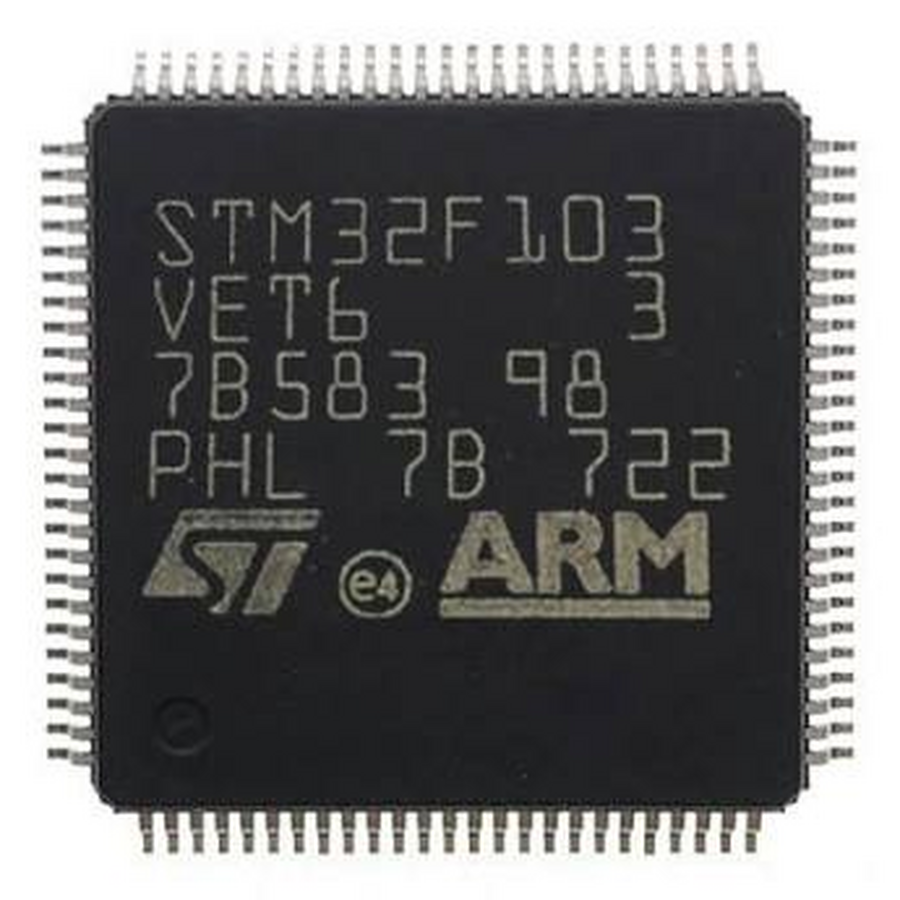
\includegraphics[height=4.0cm]{figures/ch03/stm32f103vet6.png}
	\caption{IC vi điều khiển STM32F103VET6 dạng LQFP100.}
	\label{fig:control-stm32f103vet6}
\end{figure}

\begin{table}[H]
	\centering
	\caption{Thông số chính của STM32F103VET6~\cite{stm32f103veDatasheet}.}
	\label{tab:control-mcu-specifications}
	\begin{tabularx}{\linewidth}{|C{5.0cm}|Y|}
		\hline
		\textbf{Thông số} & \textbf{Giá trị} \\
		\hline
		Nhân xử lý & Arm Cortex-M3, 32 bit \\
		\hline
		Tần số hoạt động tối đa & 72 MHz \\
		\hline
		Bộ nhớ Flash & 512 KiB \\
		\hline
		Bộ nhớ SRAM & 64 KiB \\
		\hline
		Điện áp cấp cho IC & 2,0--3,6 V \\
		\hline
		Giao tiếp nối tiếp & SPI, I\textsuperscript{2}C, USART \\
		\hline
		Ngoại vi hỗ trợ điều khiển & Timer có chế độ PWM; DMA \\
		\hline
	\end{tabularx}
\end{table}

\clearpage
\subsection{Cảm biến quán tính BMI160}

BMI160 là cảm biến quán tính sáu trục, tích hợp gia tốc kế ba trục và con quay hồi chuyển ba trục. Cảm biến cung cấp dữ liệu gia tốc và vận tốc góc để xác định trạng thái chuyển động của quadrotor.

\begin{figure}[H]
	\centering
	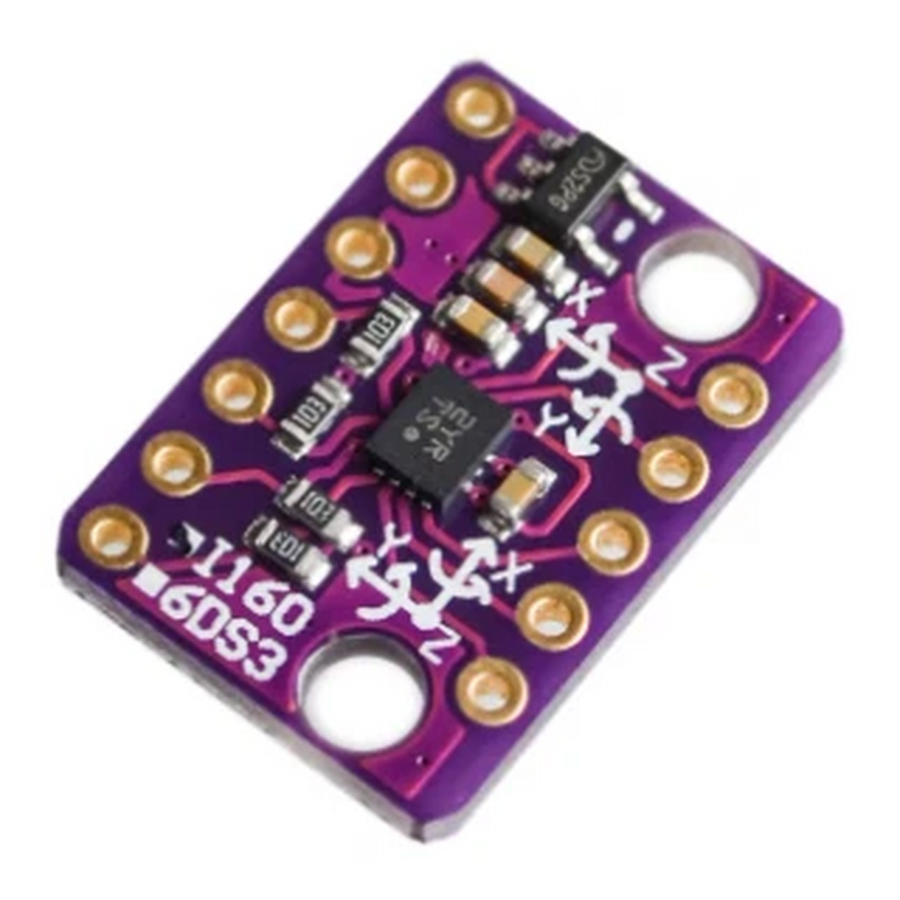
\includegraphics[height=4.2cm]{figures/ch03/bmi160.png}
	\caption{Module cảm biến quán tính BMI160.}
	\label{fig:control-bmi160}
\end{figure}

Module BMI160 trong \fref{fig:control-bmi160} đưa các chân nguồn và tín hiệu ra vị trí thuận tiện cho kết nối với bo xử lý.

\begin{table}[H]
	\centering
	\caption{Thông số chính của IC cảm biến BMI160~\cite{boschBmi160Datasheet}.}
	\label{tab:control-imu-specifications}
	\begin{tabularx}{\linewidth}{|C{5.0cm}|Y|}
		\hline
		\textbf{Thông số} & \textbf{Giá trị} \\
		\hline
		Đại lượng đo & Gia tốc ba trục và vận tốc góc ba trục \\
		\hline
		Dữ liệu đầu ra & 16 bit cho mỗi trục đo \\
		\hline
		Dải đo gia tốc lựa chọn được & $\pm2g$, $\pm4g$, $\pm8g$, $\pm16g$ \\
		\hline
		Dải đo vận tốc góc lựa chọn được & $\pm125$, $\pm250$, $\pm500$, $\pm1000$, $\pm2000\ ^\circ$/s \\
		\hline
		Giao tiếp với bộ xử lý & I\textsuperscript{2}C hoặc SPI \\
		\hline
		Điện áp nguồn VDD của IC & 1,71--3,6 V \\
		\hline
		Điện áp giao tiếp VDDIO của IC & 1,2--3,6 V \\
		\hline
	\end{tabularx}
\end{table}

Trong bảng, $g$ là gia tốc trọng trường, được dùng làm mốc biểu diễn dải đo gia tốc. Dải đo cho biết biên độ gia tốc hoặc vận tốc quay mà cảm biến có thể ghi nhận, vì thế dải đo sử dụng được lựa chọn theo mức chuyển động của quadrotor trong thí nghiệm. Các mức điện áp VDD và VDDIO mô tả nguồn cấp cho bản thân IC BMI160; khi cấp điện qua module, điện áp tại chân nguồn được xét cùng với mạch nguồn trên bo.

\clearpage
\subsection{Module cảm biến BNO055}
\label{subsec:control-bno055}

BNO055 của Bosch Sensortec tích hợp gia tốc kế, con quay hồi chuyển và từ kế, mỗi loại ba trục. Bộ xử lý tích hợp thực hiện hợp nhất dữ liệu cảm biến, cho phép xuất trực tiếp tư thế dưới dạng quaternion hoặc góc Euler~\cite{boschBno055Datasheet}.

\begin{figure}[H]
	\centering
	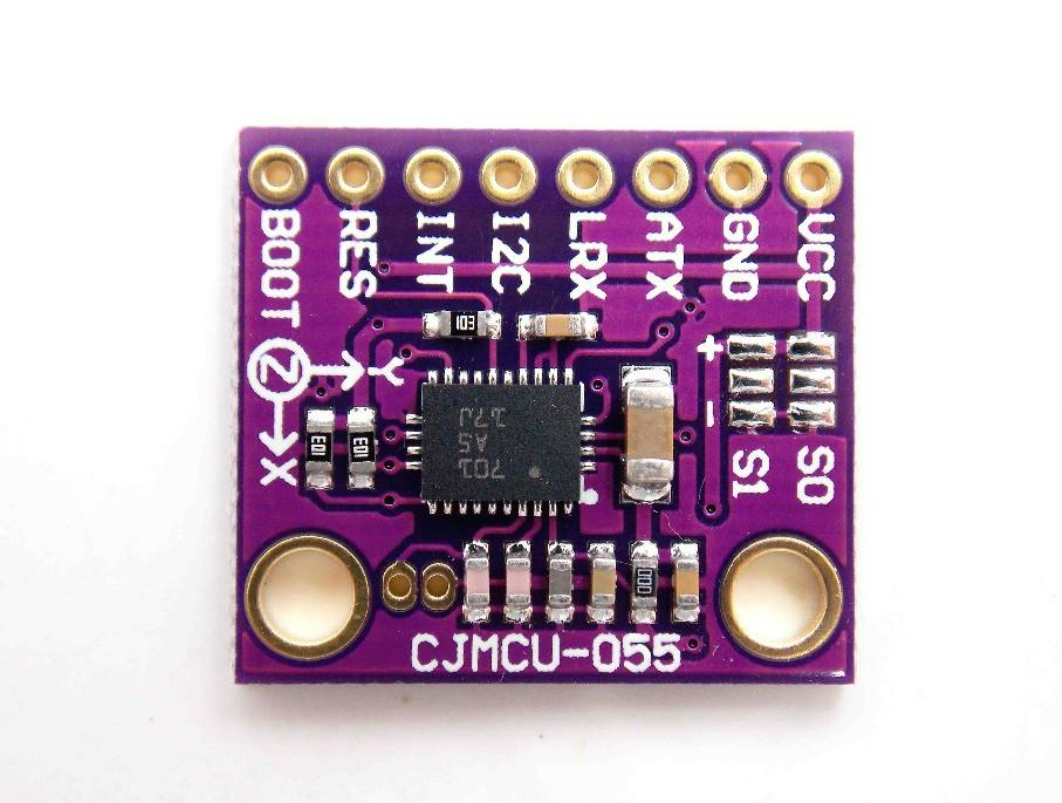
\includegraphics[height=4.8cm]{figures/ch03/cambien9truc.png}
	\caption{Module CJMCU-055 sử dụng cảm biến BNO055.}
	\label{fig:control-bno055}
\end{figure}

Module trong \fref{fig:control-bno055} đưa các chân nguồn và tín hiệu ra ngoài để kết nối với vi điều khiển. Ký hiệu hướng trục trên bo hỗ trợ xác định chiều lắp và quy đổi dữ liệu về hệ trục thân của quadrotor.

\begin{table}[H]
	\centering
	\caption{Thông số chính của IC cảm biến BNO055~\cite{boschBno055Datasheet}.}
	\label{tab:control-bno055-specifications}
	\begin{tabularx}{\linewidth}{|C{5.0cm}|Y|}
		\hline
		\textbf{Thông số} & \textbf{Giá trị} \\
		\hline
		Thành phần cảm biến & Gia tốc kế, con quay hồi chuyển và từ kế; mỗi loại ba trục \\
		\hline
		Đầu ra tư thế & Quaternion và góc Euler \\
		\hline
		Dải đo gia tốc lựa chọn được & $\pm2g$, $\pm4g$, $\pm8g$, $\pm16g$ \\
		\hline
		Dải đo vận tốc góc lựa chọn được & $\pm125$, $\pm250$, $\pm500$, $\pm1000$, $\pm2000\ ^\circ$/s \\
		\hline
		Giao tiếp với vi điều khiển & I\textsuperscript{2}C hoặc UART \\
		\hline
		Điện áp nguồn VDD của IC & 2,4--3,6 V \\
		\hline
		Điện áp giao tiếp VDDIO của IC & 1,7--3,6 V \\
		\hline
	\end{tabularx}
\end{table}

Nguồn từ chân VCC của module đi qua mạch nguồn trên bo đến BNO055. Các mức VDD và VDDIO trong bảng là điện áp cấp tại IC.

\clearpage
\subsection{Tay điều khiển Jumper T20 V2}

Tay điều khiển Jumper T20 V2 tạo lệnh điều khiển thông qua hai cần điều khiển và các công tắc chức năng. Trong đề tài, thiết bị được ghép với bộ thu ELRS 2,4 GHz để truyền lệnh của người vận hành đến quadrotor. Tay điều khiển sử dụng bộ pin riêng, độc lập với pin cấp nguồn cho hệ thống bay.

\begin{figure}[H]
	\centering
	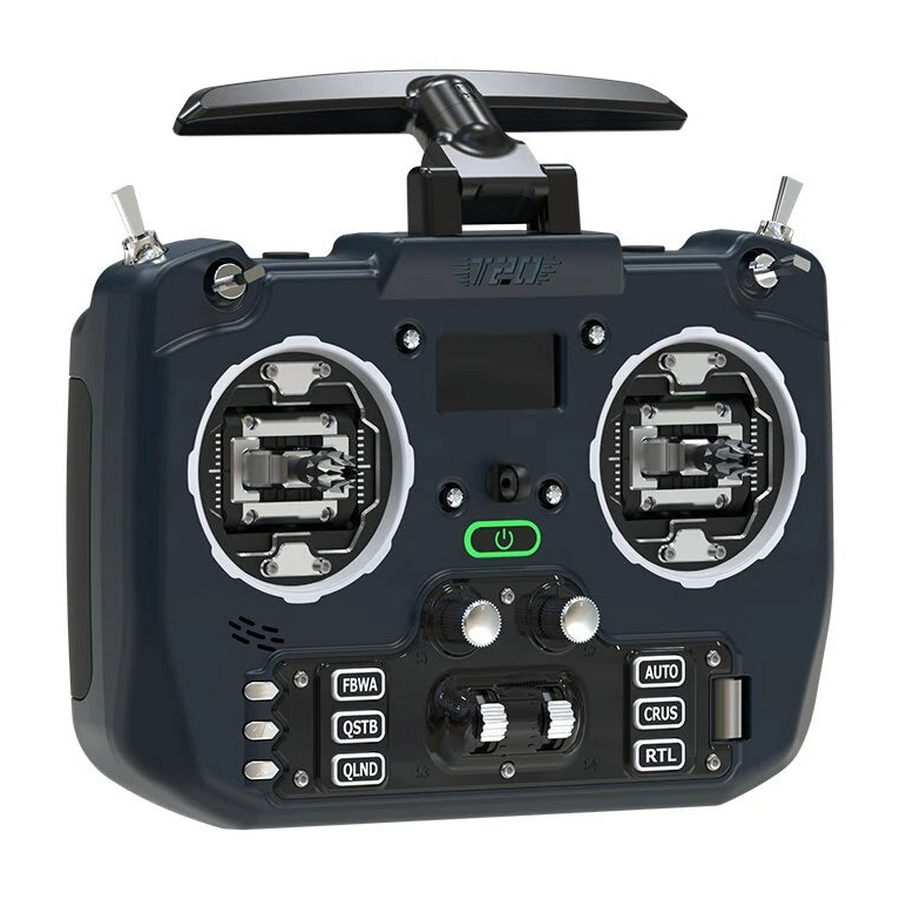
\includegraphics[height=4.8cm]{figures/ch03/jumper-t20-v2.png}
	\caption{Tay điều khiển Jumper T20 V2.}
	\label{fig:control-jumper-t20}
\end{figure}

\begin{table}[H]
	\centering
	\caption{Thông số chính của tay điều khiển Jumper T20 V2~\cite{jumperT20V2}.}
	\label{tab:control-transmitter-specifications}
	\begin{tabularx}{\linewidth}{|C{5.0cm}|Y|}
		\hline
		\textbf{Thông số} & \textbf{Giá trị} \\
		\hline
		Điện áp hoạt động & 6--8,4 V \\
		\hline
		Nguồn pin & Hai cell loại 21700 \\
		\hline
		Màn hình & OLED 1,3 inch \\
		\hline
		Độ phân giải màn hình & $128\times64$ điểm ảnh \\
		\hline
		Khối lượng công bố & 443 g, chưa bao gồm pin \\
		\hline
	\end{tabularx}
\end{table}

Các cần điều khiển cung cấp lệnh ga và lệnh thay đổi tư thế, còn các công tắc được gán cho những chức năng vận hành. Sự tương thích giữa tay điều khiển và bộ thu được xác lập theo cùng hệ liên lạc ELRS và băng tần sử dụng.

\clearpage
\subsection{Bộ thu ExpressLRS 2,4 GHz}

Bộ thu nhận lệnh vô tuyến từ tay điều khiển Jumper T20 V2 và chuyển dữ liệu kênh đến STM32. Phương án sử dụng bộ thu ELRS ở băng tần 2,4 GHz, dạng Nano để bố trí trong vùng trung tâm khung. Với loại bộ thu dùng UART, dữ liệu trao đổi với bộ điều khiển theo giao thức CRSF~\cite{expresslrsReceiverWiring}.

\begin{figure}[H]
	\centering
	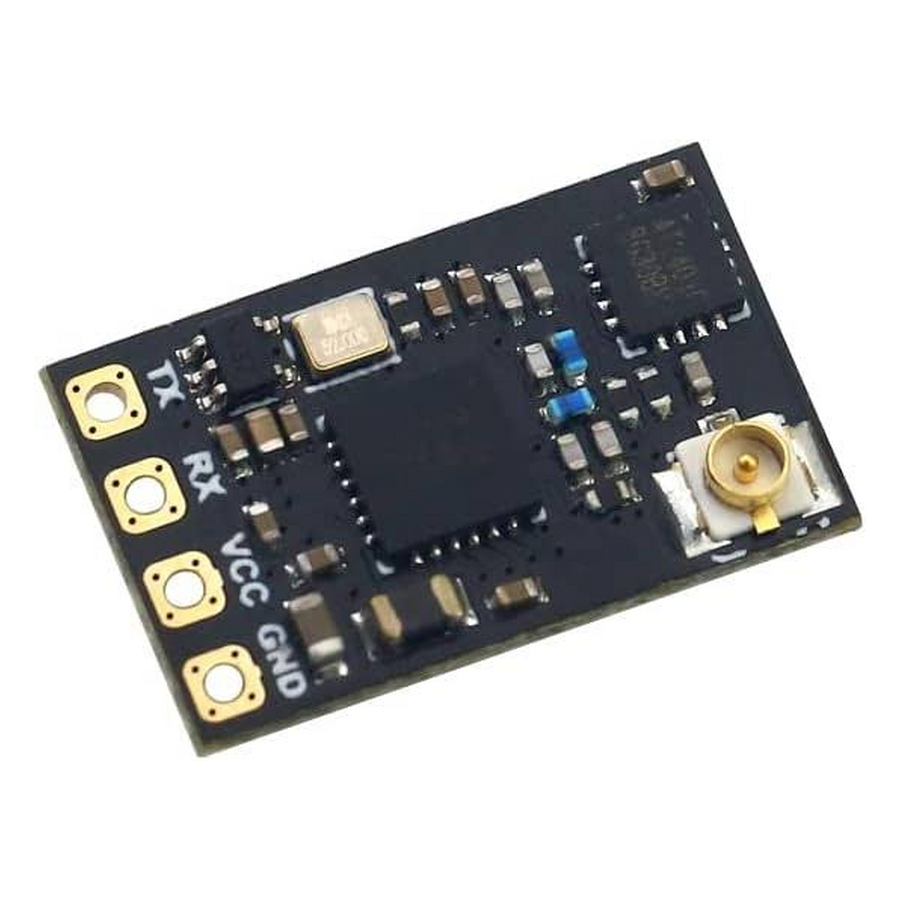
\includegraphics[height=4.2cm]{figures/ch03/elrs-24ghz-receiver.png}
	\caption{Bộ thu ELRS 2,4 GHz dạng Nano.}
	\label{fig:control-elrs-receiver}
\end{figure}

\begin{table}[H]
	\centering
	\caption{Đặc điểm của bộ thu và giao tiếp với bộ điều khiển~\cite{expresslrsReceiverWiring}.}
	\label{tab:control-receiver-specifications}
	\begin{tabularx}{\linewidth}{|C{5.0cm}|Y|}
		\hline
		\textbf{Thông số} & \textbf{Giá trị} \\
		\hline
		Hệ thống liên lạc & ExpressLRS (ELRS) \\
		\hline
		Băng tần sử dụng & 2,4 GHz \\
		\hline
		Dạng module & Nano \\
		\hline
		Giao tiếp với vi điều khiển & UART, giao thức CRSF \\
		\hline
		Các chân kết nối thể hiện trên module & TX, RX, VCC và GND \\
		\hline
	\end{tabularx}
\end{table}

Ở phía vô tuyến, bộ thu tiếp nhận tín hiệu từ tay điều khiển qua anten ngoài. Lệnh nhận được chuyển đến STM32 qua cặp chân TX và RX, còn hai chân VCC và GND cấp nguồn cho bộ thu. Như vậy, đường truyền lệnh và đường cấp nguồn có các chân kết nối riêng; điện áp cấp và dòng tiêu thụ được xác định theo loại module sử dụng.

\clearpage
\subsection{Lắp ráp cụm điều khiển}
\label{subsec:design-control-assembly}

\begin{figure}[H]
	\centering
	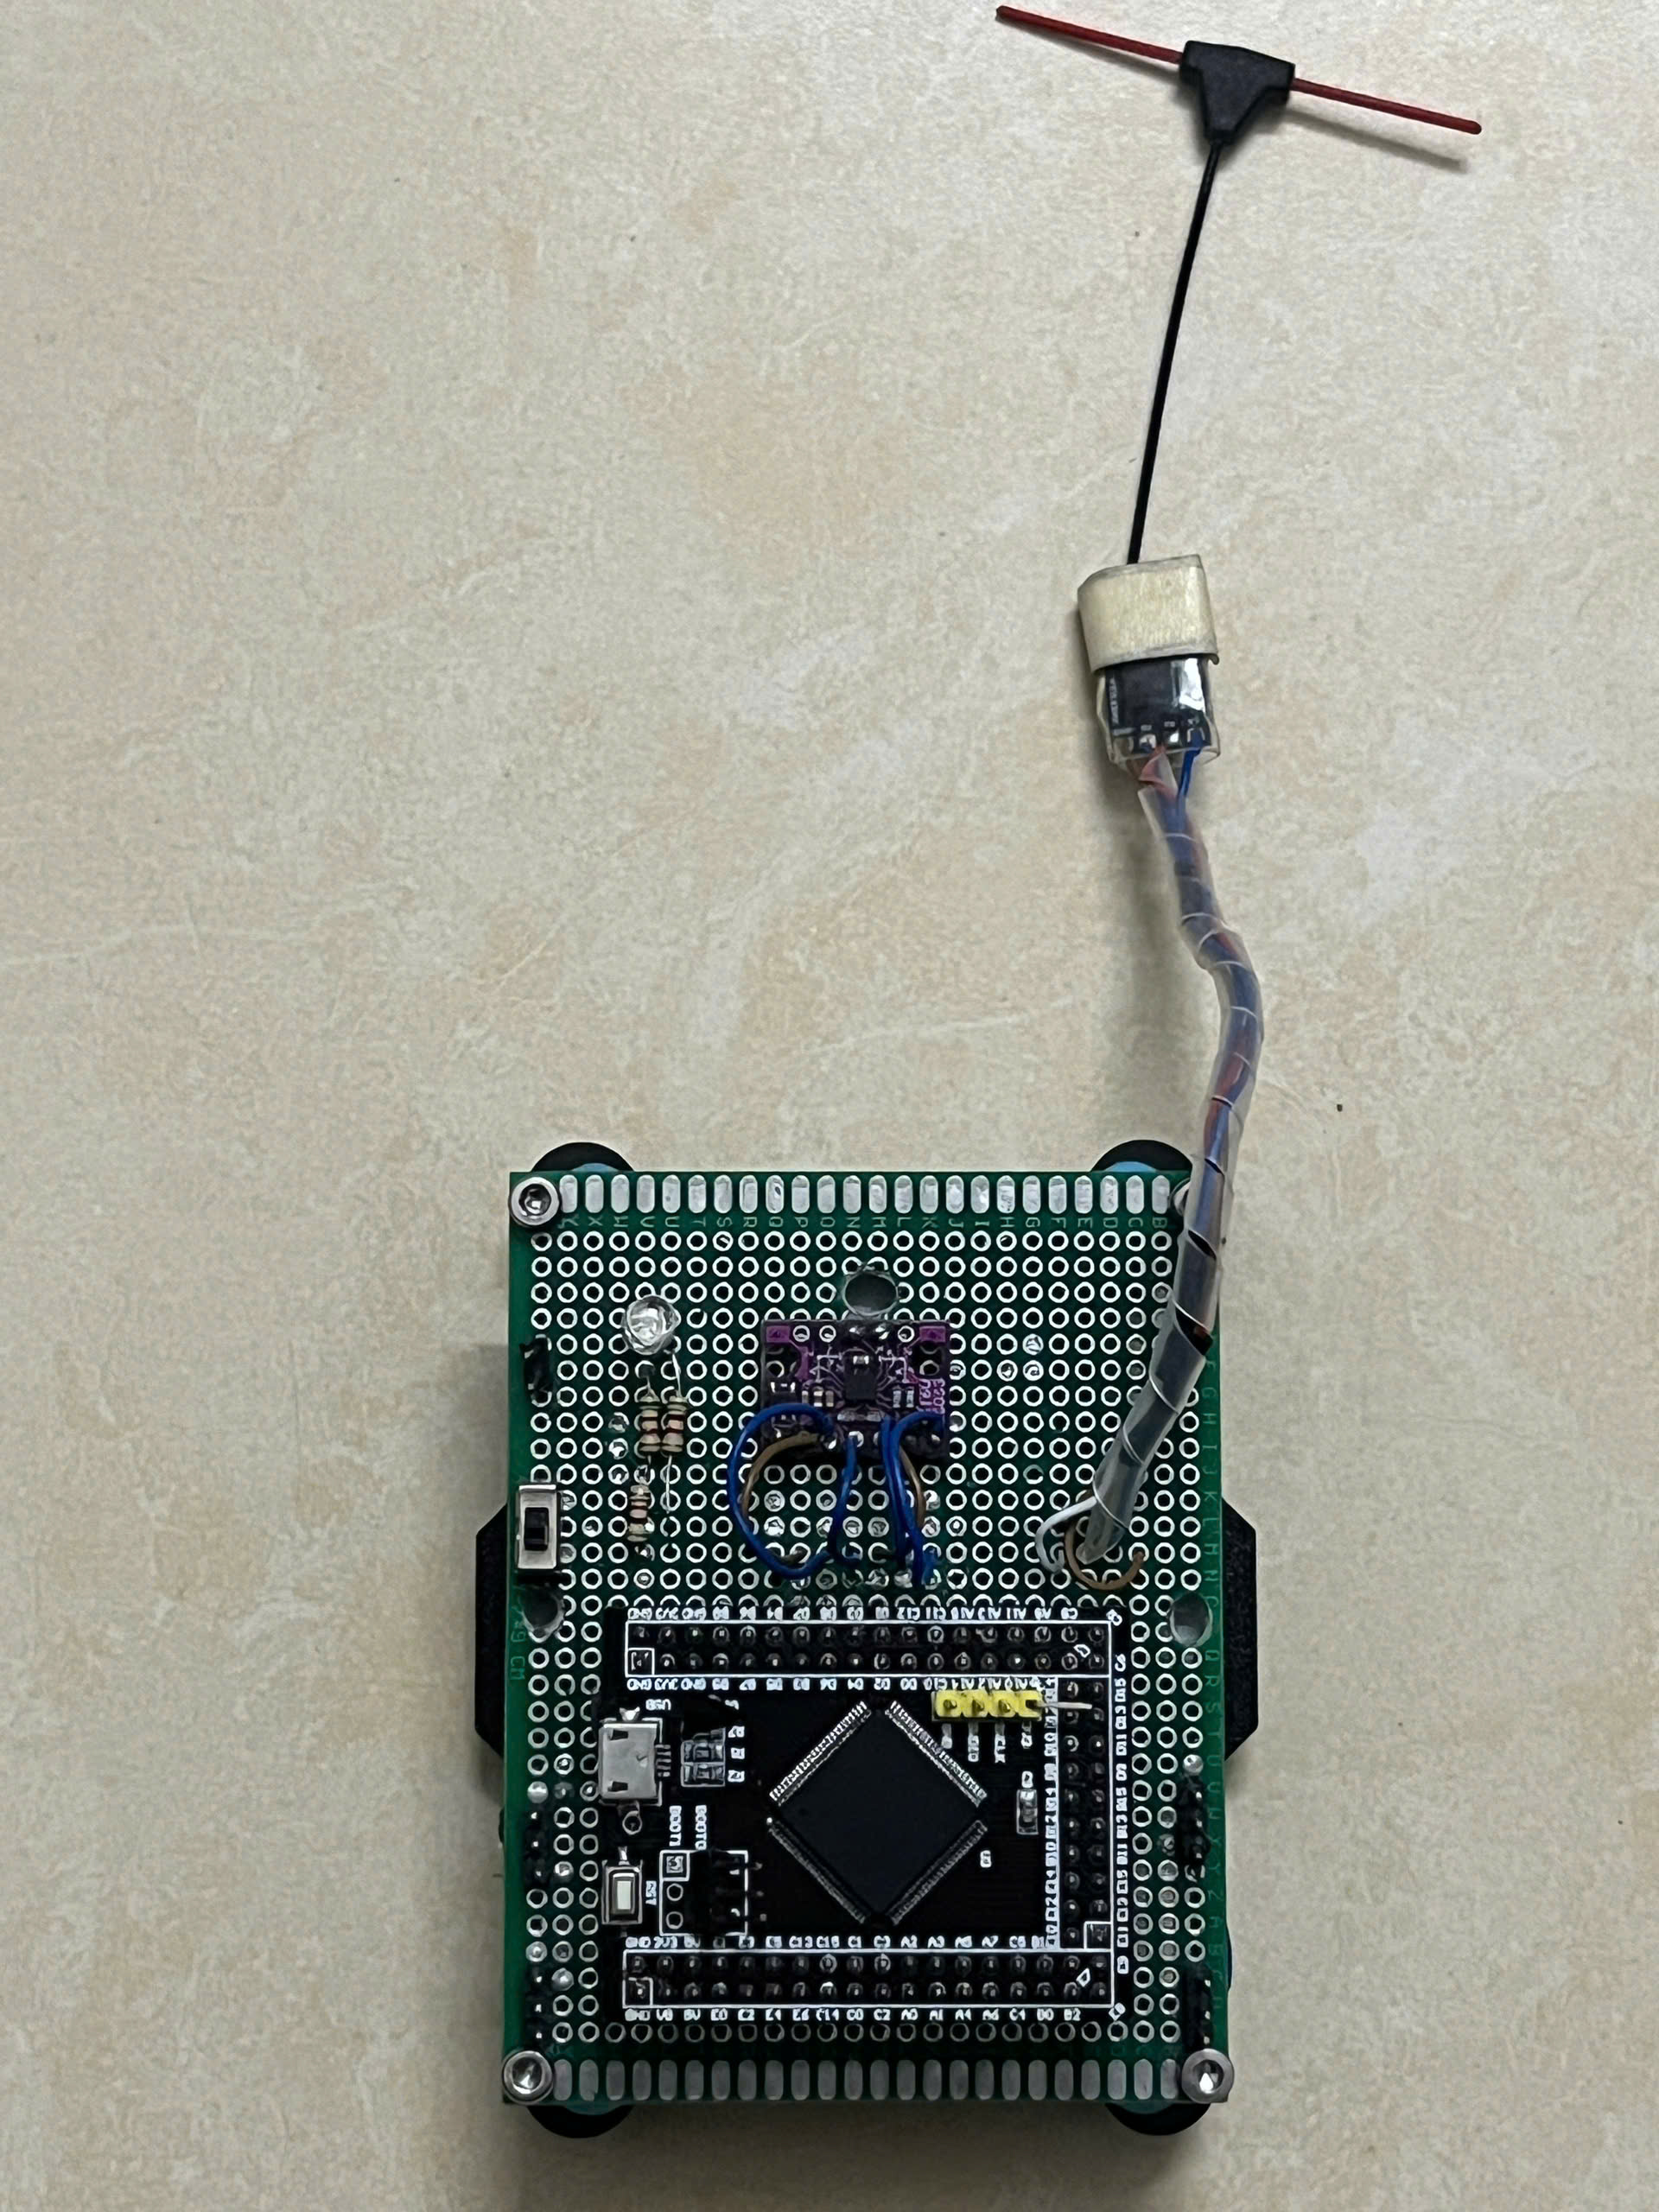
\includegraphics[trim=300bp 22bp 75bp 0,clip,width=0.85\linewidth,height=14cm,keepaspectratio]{figures/ch03/control-assembly.jpg}
	\caption{Cụm điều khiển được lắp trên bo mạch lỗ.}
	\label{fig:design-control-assembly}
\end{figure}

Bo STM32 và module cảm biến được bố trí trên cùng một bo mạch lỗ, tạo thành cụm điều khiển để lắp vào thân quadrotor. Các hàng chân cắm đưa kết nối của bo xử lý ra ngoài, còn dây nối liên kết bộ thu vô tuyến với cụm mạch. Bộ thu được bọc bảo vệ và nối với anten chữ T đặt tách khỏi bo. Các vị trí bắt vít ở góc bo tạo điểm liên kết cơ khí khi đưa cụm điều khiển lên khung.
